\fancyhead[LO]{{\scriptsize {\FA \ }我们最幸福 {\FA } 那条河}}%奇數頁眉的左邊
\fancyhead[RO]{{\tiny{\textcolor{Gray}{\FA \ }}}\thepage}
\fancyhead[LE]{{\tiny{\textcolor{Gray}{\FA \ }}}\thepage}
\fancyhead[RE]{{\scriptsize {\FA \ }我们最幸福 {\FA } 那条河}}%偶數頁眉的右邊
\fancyfoot[LE,RO]{}
\fancyfoot[LO,CE]{}
\fancyfoot[CO,RE]{}
\chapter*{14 {\FA } 那条河}
\addcontentsline{toc}{chapter}{\hspace{5mm}14 \textbf{>}\ \ 那条河}
\vspace{15mm}
\begin{flushright}
	\textcolor{PinYinColor}{\EN \huge{The\\
	River\\
	\ \\}}
\end{flushright}

\begin{figure}[!htbp]
\centering
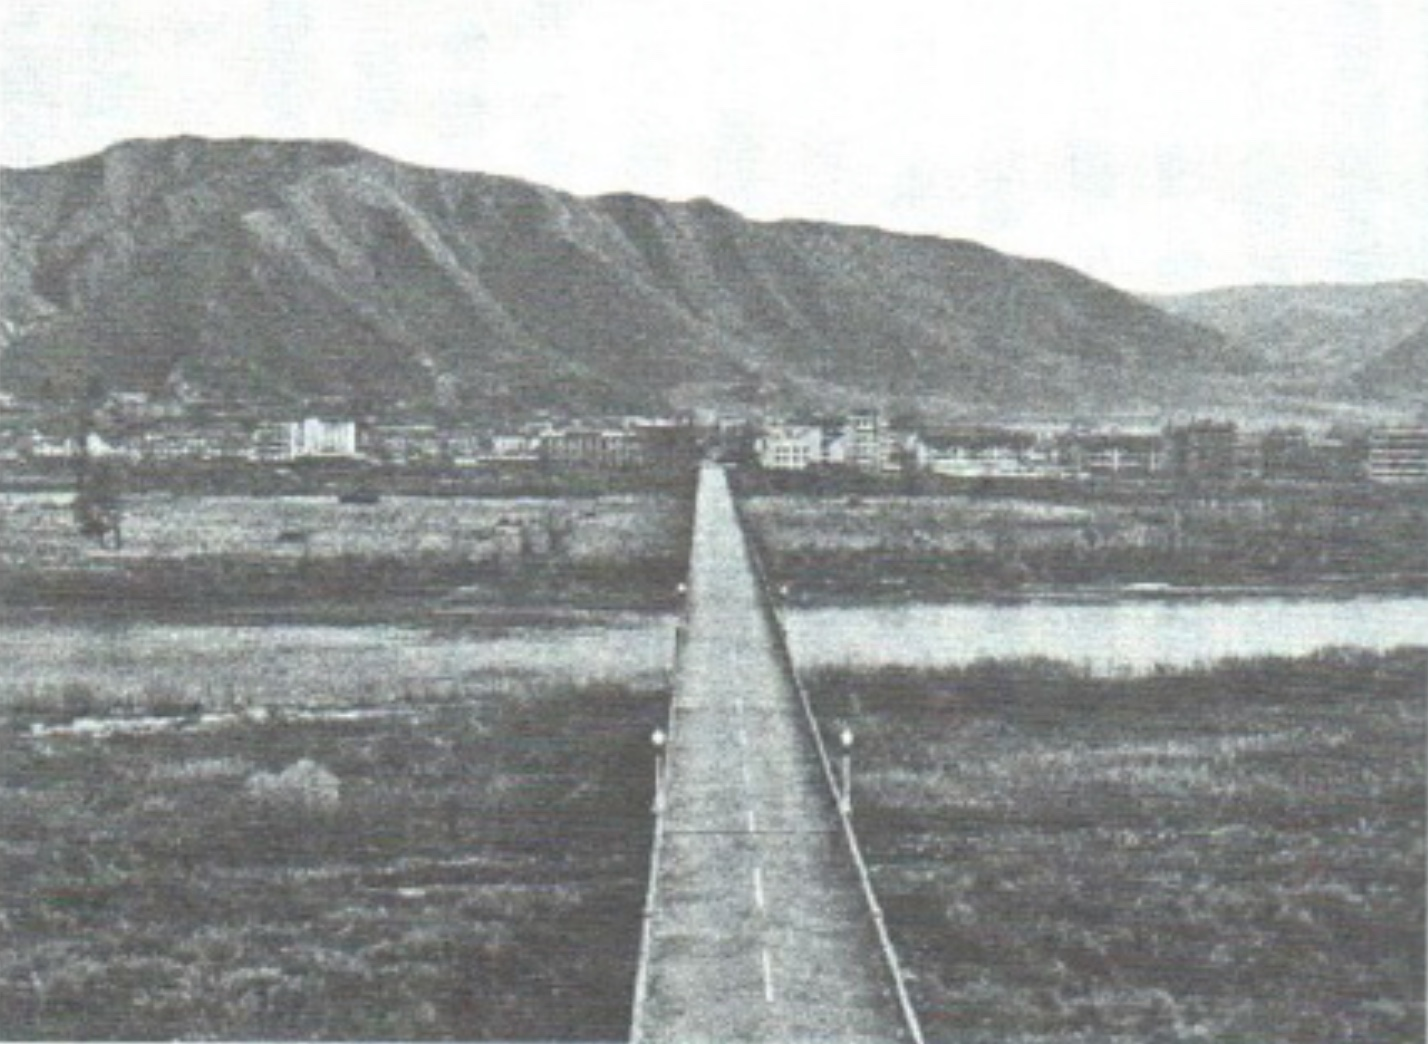
\includegraphics[width=6cm]{./Chapters/Images/14.jpg}
\caption*{从中国看图们江}
\end{figure}

\ifnum\theparacolNo=2
	\begin{multicols}{\theparacolNo}
\fi
相互之间倾诉的越少,他们的关系也就越紧张。\\

在过去,俊相和美兰会对他们的同学、同事家闲聊上数小时。当他们在黑暗中漫步,他给她回忆自己曾看过的每一部电影、每一本书,不放过任何一个情节。他给她背诗。他喜欢她那天生的好奇,他喜欢看她对一些闻所未闻的事物强装镇定的样子,她和大学里那些只知道埋头用功的女生太不一样了。现在,他读书的乐趣很大一部分来源于他随后将之复述给美兰听。在分离的数月里,俊相努力积累最好的素材,在脑子里反复预演,想象着给美兰讲述这些故事的时候,她眼睛里会闪烁着怎样的欣喜,她会如何毫无顾忌的开怀大笑。然而现在,他却对她有所保留,即使脑子里满是那些他不能与其它人倾诉的观点。\\

不是他不信任她,他觉得美兰甚至比他的直系亲属还要亲近。当其它的朋友一个个疏远时,美兰就更是他生活的中心。但是告诉她这些有什么好处呢?如果她知道了他所知道的,她会不会像自己一样,也被这些事情弄得不开心?如果她知道了南韩的富裕程度,她又怎么能继续教那些饥肠辘辘的孩子唱金日成赞歌?她为什么需要知道在中国和俄罗斯进行的资本主义改革?他很担心美兰。她的家庭成分不好,她应该比其它人更加小心自己的行为。只言片语就足以毁了她。当他们在一起,谈及她那些饿肚子的学生,他们总是用些诸如“形势”,“艰难行军”等一些委婉的词。挑的太明,可能会陷他们于要相互揭发的危险。\\

其它未曾触及的话题就是个人方面的。俊相怀疑美兰被自己1997年大学毕业后决定留在研究所的选择深深的伤害了。这样要靠破烂不堪的铁路,以及几乎陷于瘫痪的邮政,来维系这段感情就更加困难了。就算回家,相互之间的联系还是让人气馁。既没有电话,也不能在对方家里留便条。要约会,俊相就要想方设法在美兰家外面或者幼儿园里去碰美兰。有时候下暴雪,俊相要艰难跋涉几个小时,才能到幼儿园,大雪茫茫,只有将铁路线作为方向的参照。当到达的时候,他的手指几乎都冻僵了,却发现美兰今天不上班。\\

他们1年只见两次:只在寒假和暑假。在经历长时间的分离后,即使见面,还要花点时间克服一开始的尴尬。美兰变了。初次邂逅时大胆的短发早已不见。美兰现在看上去和其它北朝鲜姑娘差不多,齐肩长发,扎在脑后。他还惊奇的发现美兰开始化妆了。\\

事实是,他们现在都是羽翼丰满的成年人了。他27岁,而她25岁。很明显他们将何去何从,没有答案。\\

在俊相的一次来访时,这个话题没有任何预兆的提出来了。美兰那天早些时候刚刚参加了自己一个同学的婚礼。喜宴之后,她和俊相在她家后面见面,然后又来到了那个温泉度假村。那是个晴朗的夜空,四周一片寂静。他们在树下的小径漫步,倘佯于假山、瀑布、映景池之间。他们在最喜欢的长椅上坐下,从那里可以看到月亮挂在群山之上。\\

美兰向俊相打趣的说着婚礼和她朋友的新婚丈夫。\\

“我不知道人们为什么要这么年轻就结婚。”俊相突然插话。他最近读了一首朝鲜古典诗歌,这首诗在他脑海里,引起巨大的共鸣。他找出年轻新娘不幸的段落。\\

\begin{quote}
	\begin{spacing}{0.5}  %行間距倍率
		\textit{{\footnotesize
				\begin{description}
					\item[\textcolor{Gray}{\FA }] 如果在山间突遇猛虎,它会比婆婆更可怕吗?
					\item[\textcolor{Gray}{\FA }] 彻骨的冰霜会冷过公公的冷漠吗?
					\item[\textcolor{Gray}{\FA }] 即使是被你猛踩而爆裂的豆荚,它看你的眼神也不如小叔子的目光,那么肆意。
					\item[\textcolor{Gray}{\FA }] 不,即使最辣的辣椒也辛辣不过小媳妇的生活。
				\end{description}
		}}
	\end{spacing}
\end{quote}

俊相想这首诗风格颇为调侃。美兰也被逗的哈哈大笑,但是笑过之后她却沉默了;他不知道是不是她把这当成是他的一个暗示。\\

实际上,俊相对婚姻没有考虑太多,或者至少他不太愿意去考虑。一方面,他不敢想象自己会同美兰以外的人结婚,即便是同她的婚姻会堵上自己通往劳动党之路也在所不惜。入不了党,他就很难在平壤的大学里谋得一份固定工作。但是那是在当前情况下。如果他离开北朝鲜呢,和她一起?如果北朝鲜政权垮台呢?俊相前一天晚上从电视里得知,北朝鲜是当前世界上唯一的一个这样的共产政权,可能除了古巴。正如1989年柏林墙被推倒、两德统一,有朝一日朝鲜也可能统一。每次,当他在大街上走过叮满苍蝇的尸体或者看到污秽不堪、濒临死亡的孩子,他都觉得这个政权的末日快到了。他们就像生活在战争之中的国家,各种灾难不停的从四面八方袭来。在这样的条件下,俊相只能得过且过,甚至都不能对下一周做出什么计划,更不会想到婚姻了。\\

一瞬间,对自己、对美兰以及对他们现在不快乐生活的沮丧之情占据他的身体。他没什么心情继续背诗。他知道再多的话,也仅仅是聊以自慰。他做出个前所未有的大胆之举:把她搂过来,吻了她。\\

至少这是个吻。虽然嘴唇只是在美兰的面颊上比轻碰多了那么一点,在碰到达美兰的嘴唇之前就分开了,但这也是他们以前不曾有过的,是最亲蜜的身体接触。他们认识13年了、约会了9年,除了牵手什么也没有。\\

美兰看上去吓坏了。她好像不是生气,而是紧张。她突然从长椅上站起来,并示意他也这么做。\\

“好了。”她说。“我们走走吧。”\\

美兰被这个吻吓了一跳。虽然她对性只有最模糊的概念,但是她知道一个吻将把她带往一个万劫不复的深渊。她曾经听过女孩被男人睡的传言,还有她们惹上的是多么恐怖的麻烦。北朝鲜没有避孕措施,相反只有昂贵、危险的堕胎手术。\\

不像她不切实际的男友,关于婚姻,美兰想了很多。三个姐姐中有两个嫁人生子,她很多的高中同学也都订婚了。她不得不严肃对待自己的将来。她不认为俊相将来会娶她。\\

可以确信的一点是,她的成分已经有所改善。到90年代,金正日有比50年前在朝鲜战争中替另一边打仗的人更大的敌人需要着眼。一如幼年的伤疤,到了皮打皱的年纪就早以不记得了。污名会随着时间慢慢消退。即使在北朝鲜的法律体系下,三代以外,不洁之血也将被稀释。美兰和弟弟就被师范院校接纳。她大姐姣好的面容也战胜了不良的成分,嫁得也很好;丈夫是军队的文职人员,他们一起住在一个军事基地附近,那里周围的树林没有被破坏。她可以不断的给家里些在树林里采集到的松茸,一种珍贵东西可以用于换取其它食物。\\

然而,美兰仍然不得不接受些限制。例如,她怀疑她或者家里的其它人能不能得到居住在平壤的许可。如果和俊相结婚,他们最好住在清津。但是她觉得如果那样,她就要对俊相的牺牲负责。当见到他的时候,看着他那双学校里苦读时后,苍白、严肃的眼睛,她又担心他愿不愿意回到清津。回到这里,他可能会像他的老师们那样,能引经据典、满腹经纶,却无养活自己的一技之长,最终落得个饿死街头,终了一生。\\

然后是他的父母。她从未见过他们,但是听说过很多关于他们的事情。如果俊相要娶她,他们肯定会大发雷霆。他父亲可能会寻死;他母亲怎可能会装作一病不起。不考虑其它因素的话,俊相是个背负使命的儿子。他从不违背父母。\\

毕竟,来自日本的朝侨通常都是圈子里相互通婚。他们会帮他找个有日元的姑娘,或者他会在大学里遇见一个聪明、有教养的姑娘。美兰的这个又浪漫又爱读诗的男友和她就不是一类人。面对现实吧,她这样告诉自己。她开始想象没有他的生活回是怎么个样子。平淡无奇。没有诗歌。嫁个工厂工人或者像她爸爸那样的矿工。生孩子,永远生活在这个采矿小村庄或者最乐观住在清津。她觉得生活的大门慢慢关上了。\\

她的教师工作也近况惨淡。班上的学生从开始的50人,到现在只剩下了15个。每天早上,她害怕走进那栋破烂的建筑,她害怕想起离开的孩子临走时回头投向幼儿园那一道道悲伤绝望的眼神。孩子们再也不像以前那样开怀大笑。课堂上,没人能集中精神。学生不能,自从金日成死后,再也没有拿到过工资的老师们也不能。当美兰问园长,什么时候工资能恢复,这个女人只是笑了笑。\\

“可能当我们和南韩统一的时候吧。”她开着玩笑。\\

美兰曾想过换个工作。也许她能在市场上或者在服装厂找个工作。她如此用功才考进了师范学院,成了一名教师,才进入了主流社会。现在看起来,还是一场空。\\

美兰另外一个担心就是父亲。他现在年已60过半了,在美兰看上去,他一天天在老缩。泰宇曾经强壮的身形,随着年纪的增长也一天天佝偻下去。这让曾经自诩能将家人照顾的很好的母亲很是尴尬。现在泰宇也就终日在家转转,找些小活,有时候修修桌子或柜子,然后经常会做到一半的时候就会忘记自己在做什么。一改往常的沉默不语,现在他整日嘴不停,找任何在家的人说话,有时候甚至会自言自语。话题也都是些半个世纪以来从未提起的。他回忆在忠清南道度过的童年,还有他漂亮的妹妹们。当提及他的父亲及祖先的时候,他还颇为得意的说他们是两班(Yangban)\footnote{两班是朝鲜半岛的贵族阶级。韩国中央研究院引用20世纪统治者日本驻朝鲜统监府(总督府)统计数据,截止到20世纪30年代,一共有1685个家庭是两班贵族家庭,大部分为在地两班,即使没有做官依然控制所在地区的人口和土地,干涉地方行政。}的一支,那是个贵族。当回忆这些的时候,他的眼睛总是湿漉漉的噙着泪水。在美兰三姐出嫁的时候,他史无前例的:喝醉了。\\

美兰的父亲一直以来都因为拒绝喝酒,使得他在他那一代的北朝鲜男人当中显得格格不入。这实际是一种自我保护的机制。在60年代目睹几个朋友,像他一样都是前南韩战俘,因为酒后吐真言而惹上麻烦。而现在时过境迁,泰宇认为他用不着那么小心了。婚礼在家举行。他们都用家酿的玉米酒敬美兰的母亲。泰宇连干三杯这种烈酒。到客人都离开的时候,他开始唱小时候就会的一首伤感的南韩民歌,也不在乎会被谁听见。\\

\begin{quote}
	\begin{spacing}{0.5}  %行間距倍率
		\textit{{\footnotesize
			\begin{description}
					\item[\textcolor{Gray}{\FA }] 我过去常常抓着妈妈的手。
					\item[\textcolor{Gray}{\FA }] 然后我松开妈妈的手去够水果糕点。
					\item[\textcolor{Gray}{\FA }] 哦,我是多么怀念抓着妈妈手的感觉。
				\end{description}
		}}
	\end{spacing}
\end{quote}

美兰的父亲于1997年去世,时年68岁。当时美兰不在家,但是她弟弟陪在身边。他后来告诉姐姐们,父亲弥留时还喊着妈妈。\\

在去世的前几个月,泰宇清楚的述说着他的家庭。他坚持让他的独子记住族谱里他们祖先的名字,族谱是朝鲜人用来记录家族构成的一个记录。他是家里的独子,所以自己的儿子可以延续家族。\\

然而父亲还有一个最后的愿望却很难实现。泰宇希望将自己的死讯通知给自己在南韩的亲人。这个要求听起来就像个将死之人的臆想。\\

自从朝鲜战争后,分割了进半个世纪,南韩于北朝鲜之间既不通邮,也不通电话。红十字会也不允许传递信息\footnote{直到2000年,才有被精心选择的一些家庭参与家庭团聚,但是仅限于因战争而离散的家属。}。美兰和她的兄弟姐妹估计他们在南韩的祖母应该早就过世了,但是也没有父亲妹妹的线索。要联系在南韩的亲人看上去怎么都不可能办到。\\

美兰父亲死后的第二年,她姐姐,昭熙,急匆匆的跑回家里。她跑得上气不接下气,脸也涨得通红。她刚刚同一个能来往中国的朋友谈了谈。他认识一些人可以帮助我们联系到父亲的家人。一旦你去了中国,他建议美兰的姐姐,你只要拿电话给韩国拨个电话就可以了。\\

可能他们想试试?\\

美兰和昭熙一开始有点怀疑。你可不能信任一个不是家里人的人。这可能是那些秘密警察惯用的伎俩,设下圈套,让人们自投罗网。\\

在商量了几天之后,她们决定相信这个朋友。他有亲戚在中国,他们都会提供帮助。他认识一个人有一部卡车,可以载她们到边境;在那里有一个边境警察知道什么地方可以渡河,谁可以买通走另外一条路;他还有个表兄就在边境附近有座房子,到了那里她们就安全了。计划是美兰和昭熙一同去几天。他们只告诉了一个人,那就是他们新婚的姐姐,她发誓会保密。但是,她却实在无法保守这么大的一个秘密。她把秘密泄露给母亲,母亲却不准她们去。\\

“未出嫁的姑娘家不准单独去中国。”她下令。此时在外面很多流言,说很多北朝鲜妇女被强奸、拐走,最后被买到中国沦为妓女或者被杀害并被偷走人体器官。美兰的母亲说一不二。\\

他们又陷入家庭会议之中,商量着怎么做。美兰的弟弟坚持,作为家里唯一的男丁,他应该独自走一趟。母亲也不同意。他才22岁,是家里的宝贝,她的独子。\\

最后,有决定了。美兰、昭熙还有他们的弟弟去、母亲也去。这可是全家出动。她新婚的姐姐不想去,而且他们也不敢告诉大姐,她和丈夫孩子住在军队大院,她是绝对不会同意的。\\

虽然美兰一家从不属于最忠诚的那部分,她母亲甚至还嘲笑那些天天给画像掸灰的妇女。但是,他们也不是这个政权积极的反对者。他们之中最大胆的,后来才知道的,是美兰的弟弟。他看上去老老实实,实际上每晚都用耳机偷听南韩的广播。而其它人对时局不太关心;她们每天都忙着想办法填饱肚子,谁有闲工夫去管外面的世界。\\

相对于其它北朝鲜家庭,美兰一家在新的经济下过的还算滋润。母亲经营着个小磨坊。他们也没怎么挨饿;他们也老老实实不犯事。因而,他们没什么紧迫的理由需要逃离北朝鲜。但是机会就这样突然摆在眼前,一旦他们决定行动,那开弓就没有回头箭了。垂死之人的恍惚之语,现在成了驱动他们走向边境的动力。\\

他们要去中国去联系在南韩的亲人。然而,他们担心能不能找到他们,或者即使找到,他们愿不愿见自己。他们根本不敢想去南韩的事情。\\

所有的计划准备在几周之内就一一落实了。在她们的口琴屋里,由于忌惮墙壁太薄及那些爱多管闲事的邻居,所以任何可能走漏风声的事情他们都不在家做。他们努力保持外表和往常一样的平静。看不出有什么异常的。他们不能卖了家里值钱的东西去筹集路费。他们不能用木板把门窗钉死,以保全家当。\\

美兰在走之前,还有一项紧迫任务要完成。他们出发的前一夜,她从衣橱里拿出一个仔细捆扎的包裹。那是俊相写给她的信。她把这些信件和这么多年收到的礼物全部小心的保存起来。她曾收到过的最珍贵的礼物,那个蝴蝶形状镶着水钻的发卡,她却留下了。这些信必须销毁。在扔掉之前,她把每一封信撕得粉碎。她不想任何人知道这10年来,她和俊相一起度过的那些美好时光。除了她弟弟,和两个姐姐,没人知道这事。现在,将这段浪漫保密比以前更为重要了。\\

美兰告诉自己,他们就是做个短途旅行,去打个电话而已,但是内心里,她知道很有可能再也回不来了,不论在南韩的亲戚是不是接纳他们。一旦他们走了,他们就会被宣布成为叛国者。“在党的关怀下,你接受了教育,你居然还背叛祖国。”她几乎都能听见党委书记在耳边这么说。她不想让俊相有负罪感。她走了之后,他的日子会同往常一样。他可以去找个适合的妻子,加入劳动党,然后在平壤作为一个科学家度过余生。\\

他会宽恕我的,他会理解的,她告知自己。这样也是为他好。\\

第二天早上,美兰动身了,只随身背了自己的背包。她骑上车,和往常一样很随意的同母亲、弟弟挥手再见。计划是每个人分头离开家,以避免引起注意。晚些时候,她母亲会在邻居家门口露面,同他们打个招呼,说要去出嫁的女儿家1-2周,帮忙照看孩子。这会给他们在警察注意到他们失踪前争取些时间。\\

他们在清津碰头,在哪里美兰的姐姐有个公寓。美兰和姐姐徒步出发去找能载他们去中国边境的那个卡车司机。美兰表现的出奇的镇定,每一步都像是纯自然的,好像她做着她应该做的,完全没有考虑到这些行为的后果。但是,当她同昭熙一起走着的时候,她恰巧扫了一眼街对面,突然她感到心脏停止了跳动。\\

她看见俊相在对面的方向走着,或者至少看上去是他。美兰的视力很好,所以即使是6车道的马路对面,她也能发誓那一定是他,即使现在是10月,他应该在大学的研究所里。她第一的反应就是想穿过马路去拥抱他,当然在大庭广众之下,她不能这么做。但是,她有太多事情要向他倾诉。她想他知道,她很担心他。她希望他能过的好。她还要感谢他曾给予的鼓励,鼓励她考入师范学院。她想告诉他,他对生活的热情也鼓励着她积极去面对自己的生活,包括当下正要做的事情。如果她的行为短期内伤害了他,她感到十分难过,但是……她强迫自己不要想了。这些话刚刚浮现在脑海里,她马上就意识到她收不住嘴,她会泄露秘密的。这样会危及全家,而且如果他知道了的话,对他也不好。\\

她在自己这边没有停住脚步,但每个几秒就回过头看看,直到那个也许是也许不是俊相的人消失在人群之中。\\

他们静静的坐在卡车后货箱里,前往茂山,这个美兰父亲在朝鲜战争后作为战俘被送往的城市。现在的茂山几乎成了个鬼城,煤矿、工厂都关了门。但是在毫无生气的外表下面,却是暗流涌动,这里成了走私者的乐园。这个镇子坐落于图们江江面最窄的一段,同会宁市和稳城郡一道,发展成非法越境中国的一个枢纽。非法越境在北朝鲜是个发展很快的行业,可能是北朝鲜唯一增长的行业。这个卡车司机就是专门带这些没有护照和旅行许可的人到边境的。乘火车是想都不要想的,那里旅行证查的非常严。\\

如果有人看到他们一家,没人会怀疑他们在逃离自己的家。他们将自己最好的衣服穿在了日常穿着的下面,希望到了中国后,不要显得太寒酸。他们的穿著看上去也合符他们的借口──他们来茂山参加家庭婚礼。他们随身带的几件行李也只够他们来次周末短途旅行。里面也就塞了几张家庭合影,一些干海鲜、鱼、墨鱼、螃蟹等清津的土特产。这些不是给自己吃的,都是用来贿赂的。在去茂山的80公里的路程上,有两个检查点。早些年,没有许可他们是不敢来茂山的;但是在1998年你用吃的什么都可以换来。\\

跨境被精心选择在一个没有月光的晚上,在边防守卫最可能打瞌睡的时候行动。地点就是茂山郊外的一处,那里边防岗亭相距200米。跨界的时间、地点都是同中国那边的向导仔细协调过了的,他会在半夜过后,在河对面等着这些“包裹”\\

美兰独自一人行动。她母亲,弟弟和姐姐按照安排都先走一步。为了安全,全家人最好分开过河。因为如果单独被抓,你可以煞有介事的声称自己过去是应为肚子饿。如果走运,你可能会被轻判,也许只要在劳动营里待1年。如果全家被抓,就很明显的是有预谋的叛逃,那么惩罚就会非常、非常严厉。具体什么惩罚,美兰不知道,因为她从来没有遇见跑出来的人。她努力的让自己不要去想这些事情。\\

有个向导护送她,沿着一条平行于河道的土路,出了茂山。这时,路到一片玉米地前来到了尽头。他示意她穿过玉米地,一直朝着河的方向走。\\

“直走,不要停。”向导告诉她。\\

现在,美兰超常的镇定又发挥了作用。由于恐惧和寒冷,她的身体不由自主的打起哆嗦。10月天,还是秋老虎发威的时候,但是一到了晚上,就感到阵阵的秋风凉。树枝上只挂有有几片枯叶。光秃秃的树枝让美兰暴露无遗。最好现在就穿过待收割的玉米地,走路尽量轻,干枯的玉米秆在脚下瑟瑟作响。她肯定有人正盯着她,马上要抓住她的脖子。\\

没有任何光线做参照,要按照向导的话直走很困难。哪边才是真正的直走?河在那里?她现在是不是应该走到河边了?她怀疑自己是不是一直在玉米地里转圈。\\

然后她几乎撞上了一堵墙。它就横在自己的去路上,高过头顶,视力所及向两边延伸而去。那是堵混凝土墙,就像是监狱和军事基地的那种围墙。她落入陷阱了吗?她现在很明确她走错了路。她要离开这里。越快越好。\\

她沿着白色的墙边走向前走。边走边用手摸着墙,墙也越来越矮,最后矮到很容易就翻过去。她现在明白了,这是一堵河岸的挡土墙。她摸索着下了水。\\

秋天在朝鲜是枯水期,河流很浅,只及膝盖,但是河水却冰冷刺骨,她的脚不一会儿就麻木了。当运动鞋灌满了水后,两只鞋就像是铅做的。她忘记了向导告诉她要卷起裤腿。她陷入了淤泥。她拔起一只脚,另一只又陷进去了。一步一步的往前挪,努力使自己不要滑倒,栽进水里。一直直走,她告诉自己,向导的话一直在脑海里回荡。\\

突然,美兰觉得水退到了脚踝处。她爬上了河岸,浑身湿漉漉的,四周看了看。她在中国了,但是什么也看不到。那里没人。黑暗里,她孤零零的。她的嗓子里又涩又干,但是现在即使她能喊,她也不敢。\\

现在,她完全慌了神。她回头看看身后的北朝鲜。现在她从另外一边看见那堵让她迷惑的墙。在那墙之外是玉米地,连着那条和向导分开的路。如果她能找到路,她可以走回茂山。在那里她可以搭火车回清津,第二天她就能到家。她可以回去幼儿园继续教书。俊相也不会知道她几乎就跑了。一切都好像是没有发生过。\\

当她胡思乱想的时候,她听见树丛后一阵沙沙声,然后是个男人的声音。\\

“Nuna,nuna。”\\

是朝鲜语“姐姐,姐姐。”那是她弟弟在喊她。\\

她伸手抓住他的手,永别了,北朝鲜。\\
\ifnum\theparacolNo=2
	\end{multicols}
\fi